\chapter{Раси}
%Метаправила:  \\
%Качествата струват съответно по 1 и -1 точка за положителни и отрицателни качества.  \\
%Правото на две расови умения на 5, без да е нужно да покриват изисквания, без точките да се плащат от (5 * Ум), струва една точка.  \\
%Човеците имат всикчи показатели 1 - 10.  \\
%За всеки 3 точки по максимуми над 10, расата струва още една точка.  \\
%За всеки 5 точки по минимуми, расата струва една точка по-малко.  \\
%\\
\begin{multicols}{2}
\race{Homo Sapiens}{0}
{Доплавали на Ендивал от юг преди 4 века и провъзгласили Каланор и обширната Луседум Терея.}
{1 - 10}{1 - 10}{1 - 10}{1 - 10}{няма}{няма}

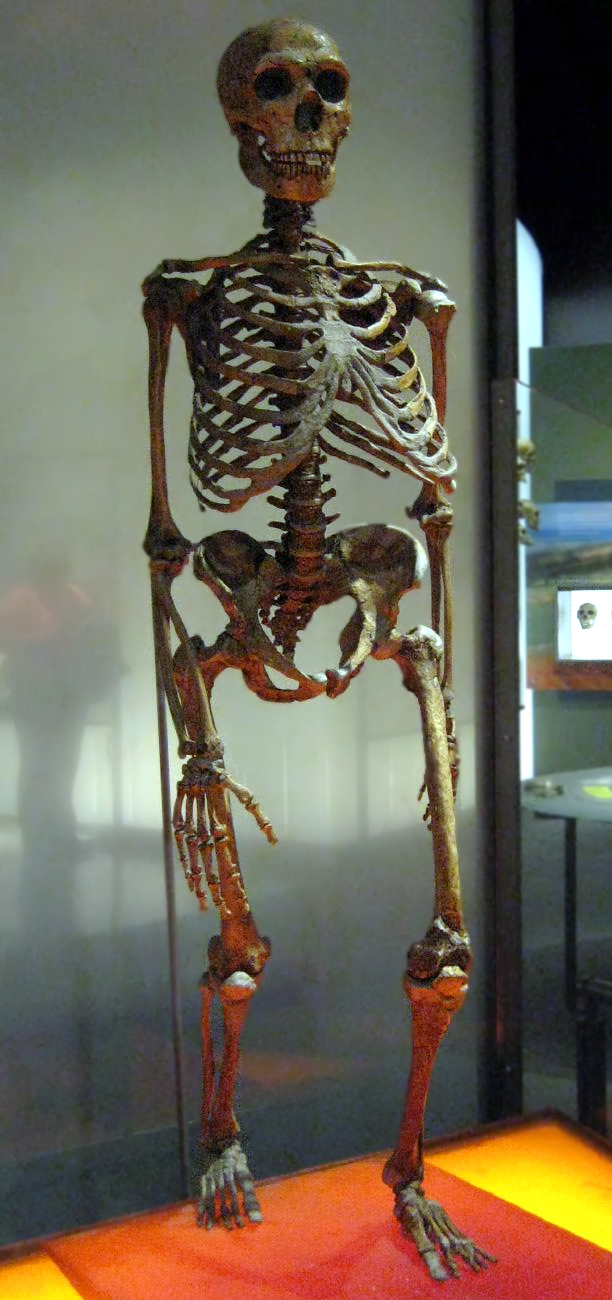
\includegraphics[height=0.25\textheight]{neanderthal1}
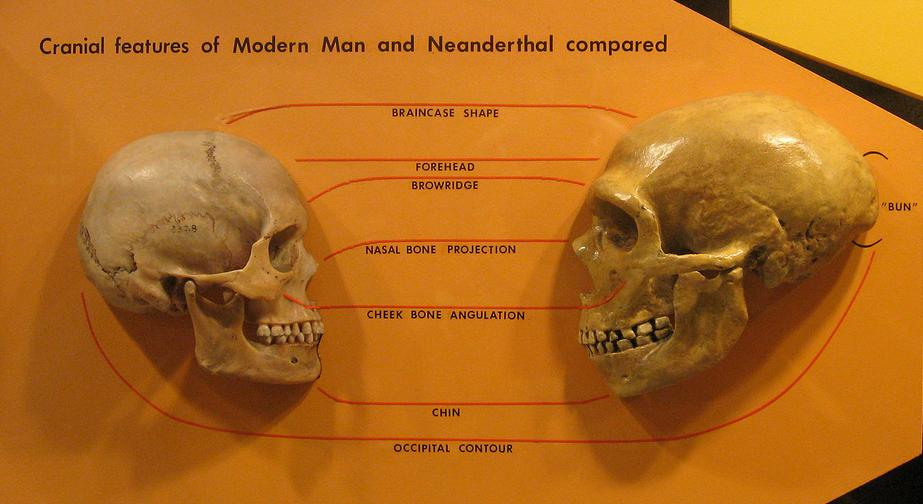
\includegraphics[height=0.25\textheight]{neanderthal2}
\race{Неандерталец}{1}
{}
{1 - 12}{1 - 11}{1 - 10}{1 - 10}
{няма}
{
Каменоделство(С)
Лов(Л)
Тичане(Л)
Копие(Л)
Промъкване(Л)
Билкарство(У)
}

\race{Джудже}{2}
{Местно население на Ендивал, което след пристигането на хората се разединява на три, а после на четири, кралства.}
{6-15}{1-8}{1-12}{1-8}{Виждане в тъмнина}
{
Джуджешки език(У);
Каменоделство(Л);
Боравене с брадва/чук(Л);
Металургия(У);
Ковачество(С)
}

\race{Елф}{4}
{Първите жители на Ендивал, сега са изтласкани до най-западните гори на континента.}
{1-8}{6-15}{1-15}{1-12}{Неспящ; Нестареещ}
{
Елфичеки език(У);
Лък(Л);
Катерене();
Магия - по избор(У);
Оцеляване в дивото(У)
}

\race{Върколак}{3}
{Създадени от Хазерот като по-съръшена раса от елфите.}
{6-16}{1-10}{1-10}{1-10}{Силна имунна система}
{
Оцеляване в дивото(У);
Вълчи език(У);
Човешки език(У);
Магия-огън(У);
Спринт(С)
}

\race{Здрачник}{4}
{Пришълци броени години преди човеците. Изтласкани да владеят горите от желязно дърво и търговията в Ендивал.}
{1-8}{1-15}{1-10}{6-16}{Изчезване в сянка}
{
Катерене(Л);
Оцеляване в дивото();
Търговия(Х);
Акробартика(Л);
Здрачничрски език(У)
}

\race{Немъртъв}{2}
{Когато немъртвите слуги станали често срещани, достатъчно от тях успяли да заменят връзката за управление от господаря си с връзка за управление към друг немъртъв.
Така те били способни да действат по собствена воля и да завладеят малко краство в северен Ендивал.}
{1-14}{1-9}{1-10}{1-4}
{
Усещане на живот (30 метра);
Телепатия;
Нестареещ;
Уязвими в ярко слънце (всчики хвърляния -10)
}
{
Магия-некромантия(У);
Поклонничество-Смърт(Х);
Строителство(У);
Тактика(У); %??
Език на немъртвите(У)
}

\race{Ниог}{5}
{Тези антропоморфни птици владеят сръчно телекинеза.
Живеят в технологични планински градове.
Са поколението на експедиция до Ендивал, която не успяла да се завърне.}
{1-6}{1-10}{1-14}{1-10}
{
Реене (може да планира по вятъра или да се издига от топли течения)
Отлитане (може да отлита и каца верикално)
Телекинеза (може да манипулира предмети до (Ум) метра със силата на една ръка и Ловкост 1)
Телекинетична сръчност (хаптична обратна връзка, както и фин контрол върху движенията)
}
{
Староендивалски език(У);
Астрономия(У);
Архитектура(У);
Употреба на обсадни оръжия(У);
Тaктика(У)
}

\race{Орк}{-2}
{Едри, раздразнителни и тъкмозелени на цвят.
Живеят в планински села и се препитават от лов и бандитлък.}
{1-16}{1-8}{1-6}{1-4}
{
Жажда за кръв %???
}
{
Език на гоблините(У);
Боравене с брадва(Л);
Оцеляване в дивото(У);
Строеж на лагер(У);
Проследяване в дивото(Л)
}

\race{Гоблин}{-3}
{Една от малкото раси, която успешно съжителства с орките.
Пристигнали заедно на Ендивал преди 12 века през подземен тунел.}
{1-6}{1-8}{1-8}{1-9}
{
Ранна старост
}
{
Език на гобилините(У);
Скриване от поглед(Л);
Капани(Л);
Плуване(С);
Катерене(Л)
}

\race{Драконит}{4}
{Човек с драконова кръв във вените си.
Драконитите живеят в малки, но строго регулирани племена, по склоновете на вулкани но и навсякъде, където е горещо.
Манюто им включва малки количества сяра и фосфор (няколко щипки на ден).}
{5-13}{1-10}{2-13}{1-10}
{
Неуязвимост от огън
Нестареещ
}
{
Език-драконски(У);
Магия-огън(У);
Магия-пазене(У);
Двуръчен меч(Л);
Древни легенди(У)
}

\end{multicols}
